\documentclass[11pt]{article}
\usepackage[letterpaper,landscape,margin=0.65in]{geometry}
\usepackage{booktabs,graphicx}
\setlength{\parindent}{0pt}
\setlength{\parskip}{6pt}
\begin{document}
\begin{center}\Large\textbf{Risk-survey responses, preference distance, and group rationality}\end{center}
\textbf{Exploratory associations.} Higher reported similarity to hypothetical own choices is associated with lower
preference distance and modestly higher group CCEI and CEIV. Cooperation scores have near-zero Pearson correlations,
but small positive rank correlations with group CCEI and CEIV. Reports about whose suggestions prevailed distinguish
preference distance much more clearly than group rationality.

\begin{center}\small
\begin{tabular}{llrrrr}\toprule
Survey & Outcome & $N$ & Pearson $r$ ($p$) & Spearman $\rho$ ($p$) & Adjusted slope ($p$)\\\midrule
Cooperation score & Preference distance & 2560 & -0.018 (0.317) & -0.006 (0.770) & -0.007 (0.323)\\
 & Group CCEI & 2607 & 0.007 (0.696) & 0.066 (0.001) & 0.000 (0.936)\\
 & Group CEIV & 2607 & 0.028 (0.168) & 0.044 (0.015) & 0.002 (0.484)\\
\addlinespace
Own-choice similarity & Preference distance & 2560 & -0.120 ($<0.001$) & -0.120 ($<0.001$) & -0.046 ($<0.001$)\\
 & Group CCEI & 2607 & 0.077 (0.001) & 0.135 ($<0.001$) & 0.010 (0.004)\\
 & Group CEIV & 2607 & 0.084 ($<0.001$) & 0.111 ($<0.001$) & 0.008 (0.003)\\
\addlinespace
\bottomrule\end{tabular}\end{center}
\small
All available respondent-wave observations for each outcome. Higher cooperation scores run from 1 to 5;
similarity runs from 1 (very differently) to 4 (mostly similar). Adjusted slopes are index-point changes per response category
after wave and class fixed effects; these are descriptive checks, not Table 5 specifications. All $p$-values use standard
errors clustered by 64 classes. Spearman tests use average tied ranks and class-clustered rank regressions.

\begin{center}
\begin{tabular}{lrrr}\toprule
Whose suggestions were reflected? & Preference distance & Group CCEI & Group CEIV\\\midrule
Category means: $R^2$ & 0.032 & 0.003 & 0.001\\
Joint test of categories: $p$ & $<0.001$ & 0.098 & 0.339\\
\bottomrule\end{tabular}\end{center}
``Whose suggestions?'' is nominal: Mostly Partner's, Both, Mostly Mine, Neither. No ordinal correlation is imposed.

\textbf{Interpretation.} These results validate perceived alignment and influence more directly than a deliberation mechanism.
Cooperation provides weak support for the proposed story. Similarity can reflect preference agreement, influence, or an
easier task; it does not establish a discussion of preferences or stable aggregation weights. Group CCEI does not identify
constant weights, and CEIV does not identify turn-taking. Outcomes and reports were measured in the same wave.
\clearpage
\begin{center}\Large\textbf{Reported cooperation}\par
\normalsize Cooperation score (coded 1 to 5)\end{center}
\begin{center}
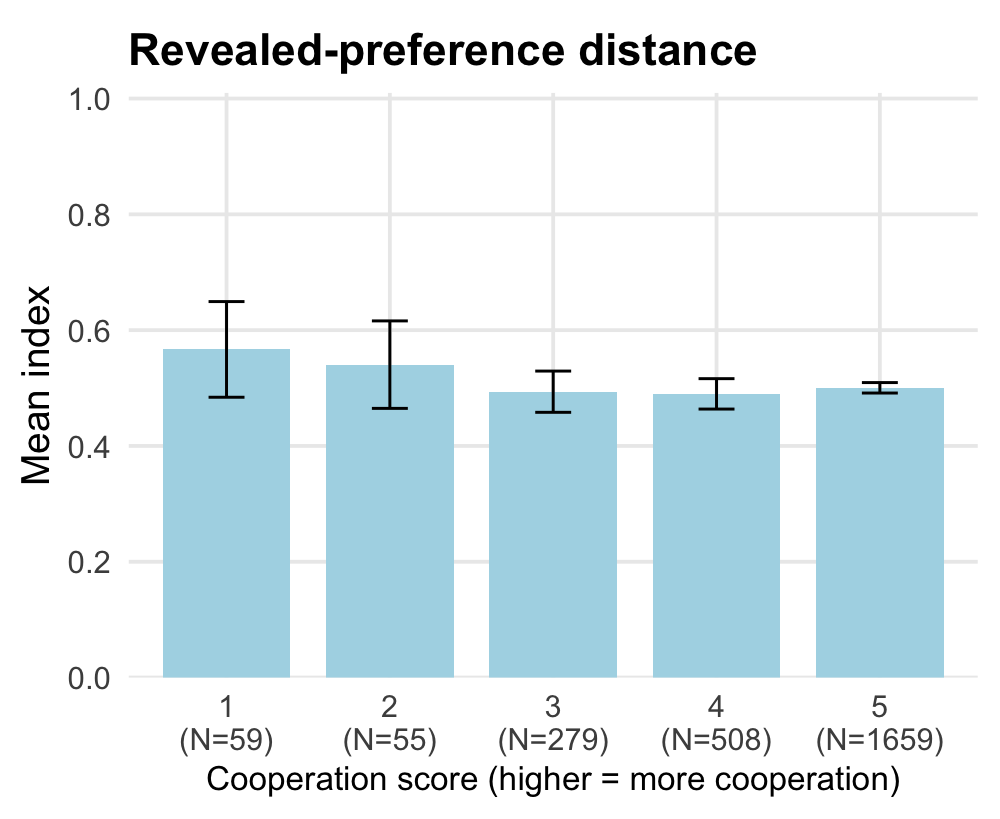
\includegraphics[width=0.326\textwidth]{cooperation.common.distance.png}
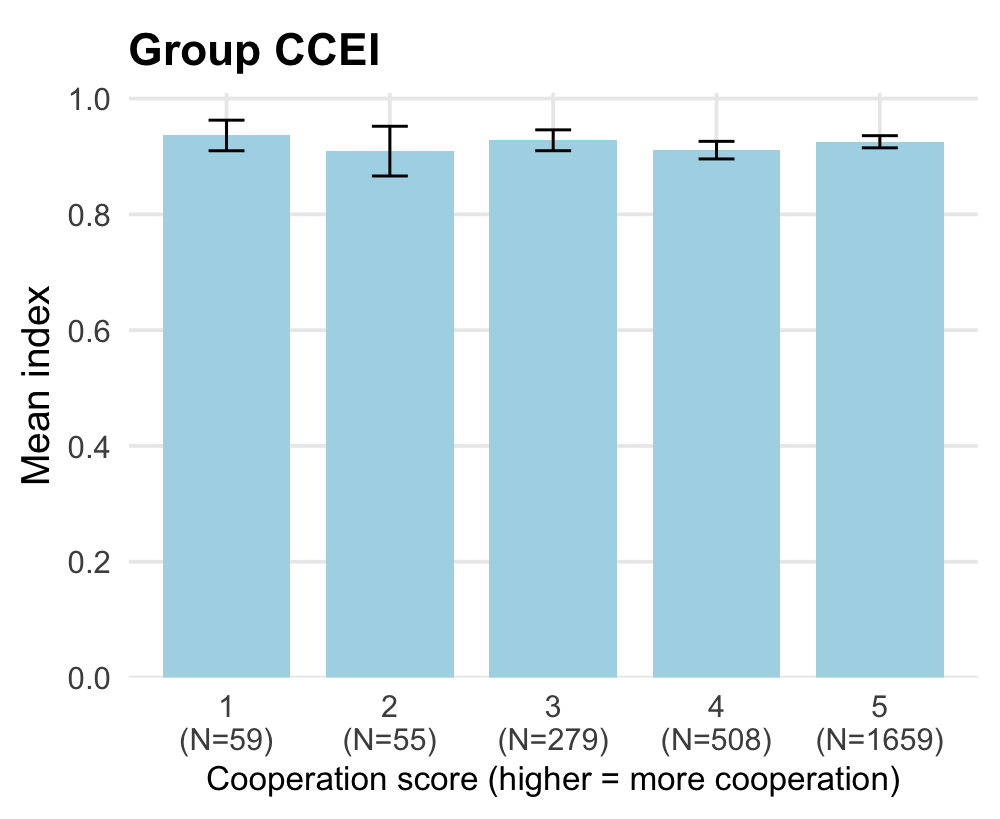
\includegraphics[width=0.326\textwidth]{cooperation.common.ccei_g.png}
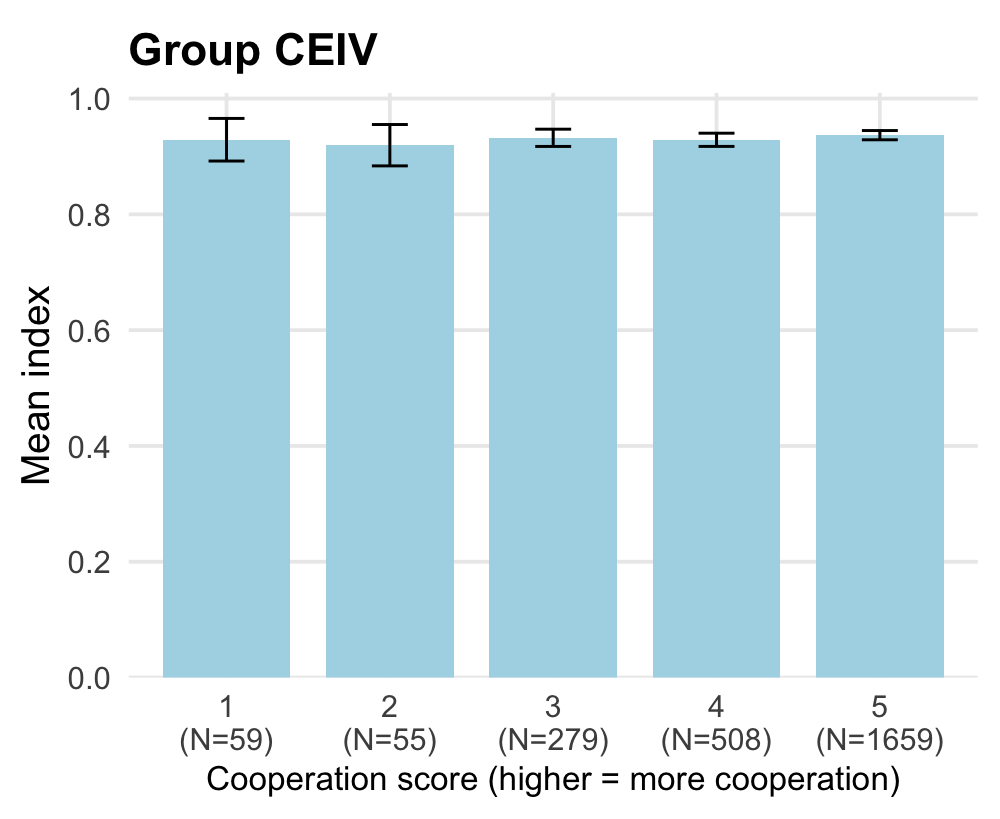
\includegraphics[width=0.326\textwidth]{cooperation.common.ceiv_g.png}
\end{center}
\small
Higher coded scores indicate more cooperation. The exact questionnaire wording and answer anchors have not been recovered, so they are not reconstructed here. The distribution is concentrated at score 5; the low-score bins are small.

\textit{Notes:} Means and 95\% confidence intervals clustered by 64 classes. All three panels use the same 2,560 respondent-wave observations (1,280 pair-waves). Group CCEI and CEIV are shared by the two members; plots sort them by each member's own survey response. Counts therefore refer to respondents, not independent groups. All panels use a common 0--1 scale.

\textbf{Reading the pattern.} Mean outcomes do not display a clear monotonic gradient. Small positive rank correlations for group outcomes coexist with near-zero linear associations.

Preference distance is the current raw normalized $I_{ig}$ used in Figure 5, with lower values indicating greater alignment. Within each pair-wave, the two defined distances sum to one; it is a relative member-to-group measure, not an absolute measure of group quality. The 48 observations without distance are excluded from these plots, while the summary correlations use all available observations for each outcome.
\clearpage
\begin{center}\Large\textbf{Similarity of hypothetical own choices}\par
\normalsize How similar would own choices have been?\end{center}
\begin{center}
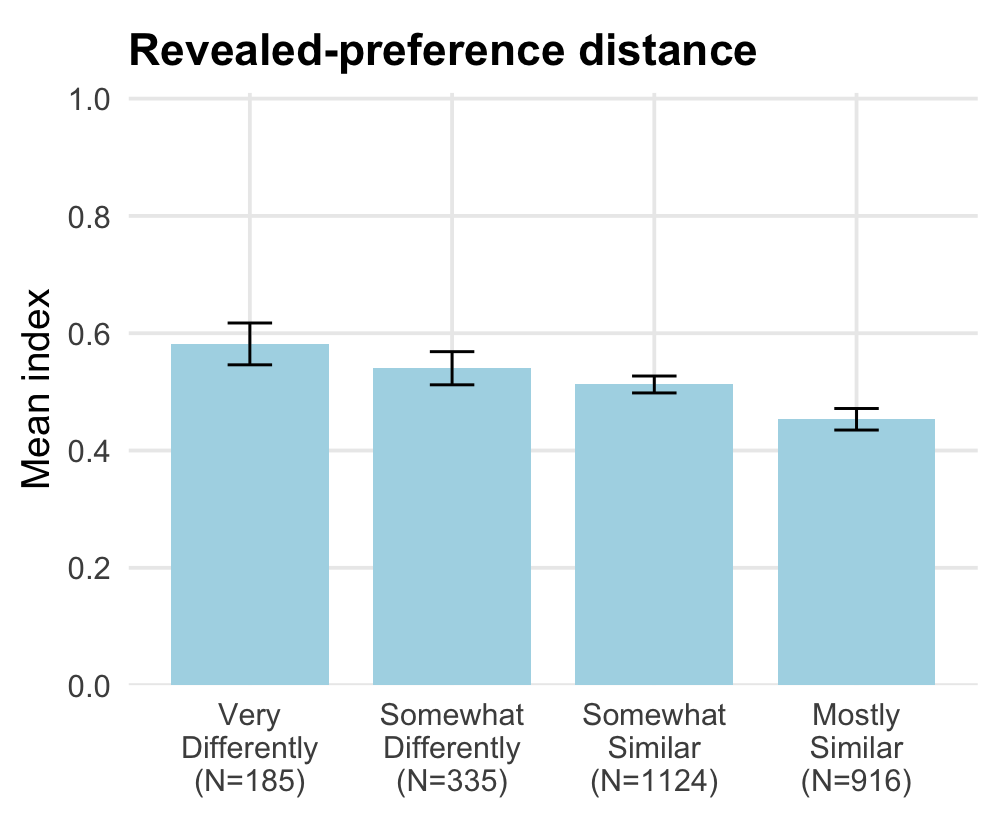
\includegraphics[width=0.326\textwidth]{similar.common.distance.png}
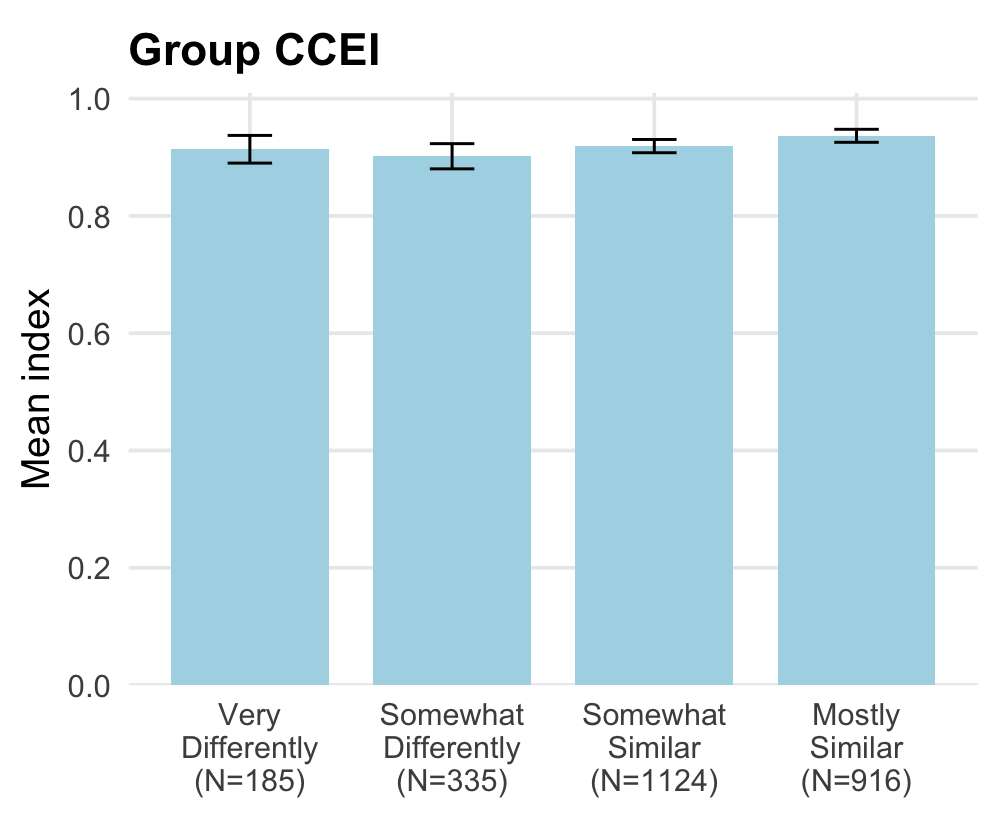
\includegraphics[width=0.326\textwidth]{similar.common.ccei_g.png}
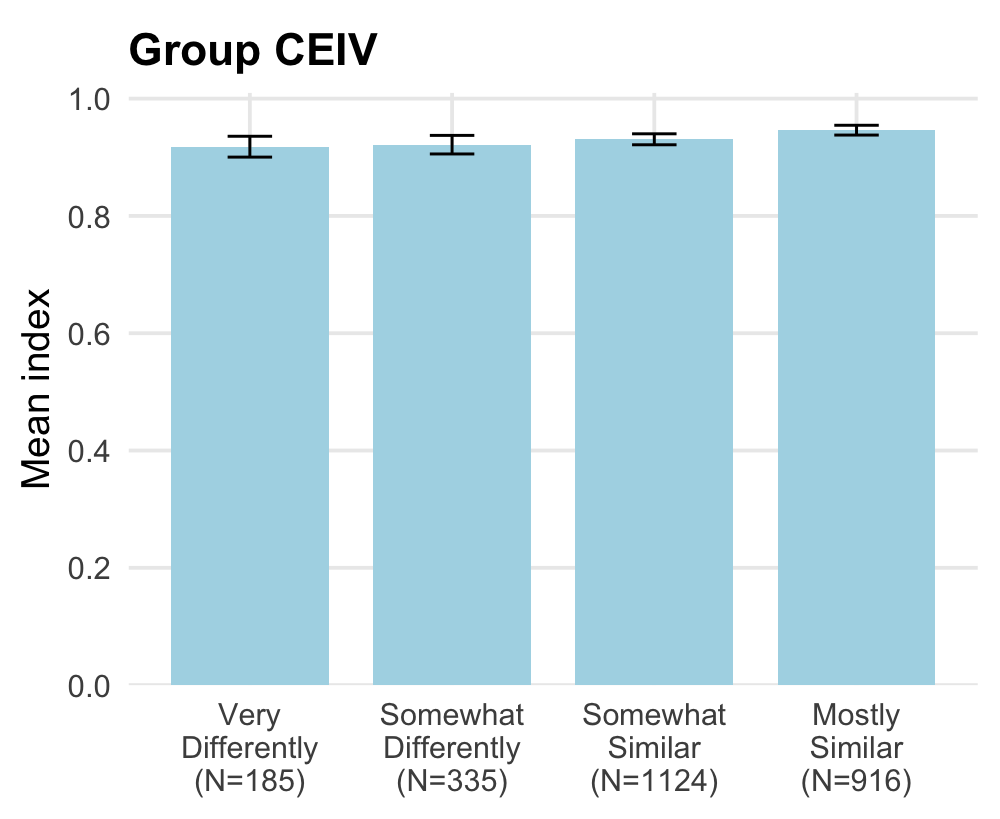
\includegraphics[width=0.326\textwidth]{similar.common.ceiv_g.png}
\end{center}
\small
Survey: If you had individually made decisions under the same choice environments as in the group experiment, how similar do you think those decisions would have been?

\textit{Notes:} Means and 95\% confidence intervals clustered by 64 classes. All three panels use the same 2,560 respondent-wave observations (1,280 pair-waves). Group CCEI and CEIV are shared by the two members; plots sort them by each member's own survey response. Counts therefore refer to respondents, not independent groups. All panels use a common 0--1 scale.

\textbf{Reading the pattern.} Higher reported similarity tracks lower preference distance and somewhat higher group CCEI and CEIV. This is consistent with agreement or alignment, but the report does not reveal the process used to reach it.

Preference distance is the current raw normalized $I_{ig}$ used in Figure 5, with lower values indicating greater alignment. Within each pair-wave, the two defined distances sum to one; it is a relative member-to-group measure, not an absolute measure of group quality. The 48 observations without distance are excluded from these plots, while the summary correlations use all available observations for each outcome.
\clearpage
\begin{center}\Large\textbf{Whose suggestions were reflected?}\par
\normalsize Whose suggestions were most reflected in final choices?\end{center}
\begin{center}
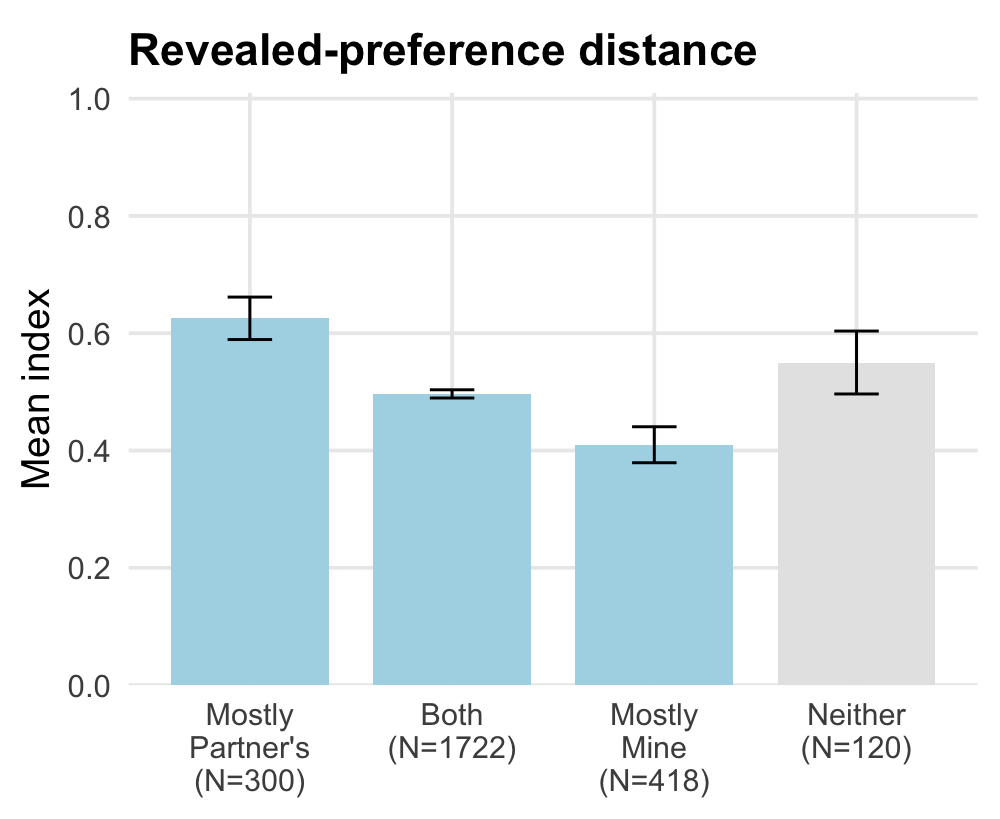
\includegraphics[width=0.326\textwidth]{whose.common.distance.png}
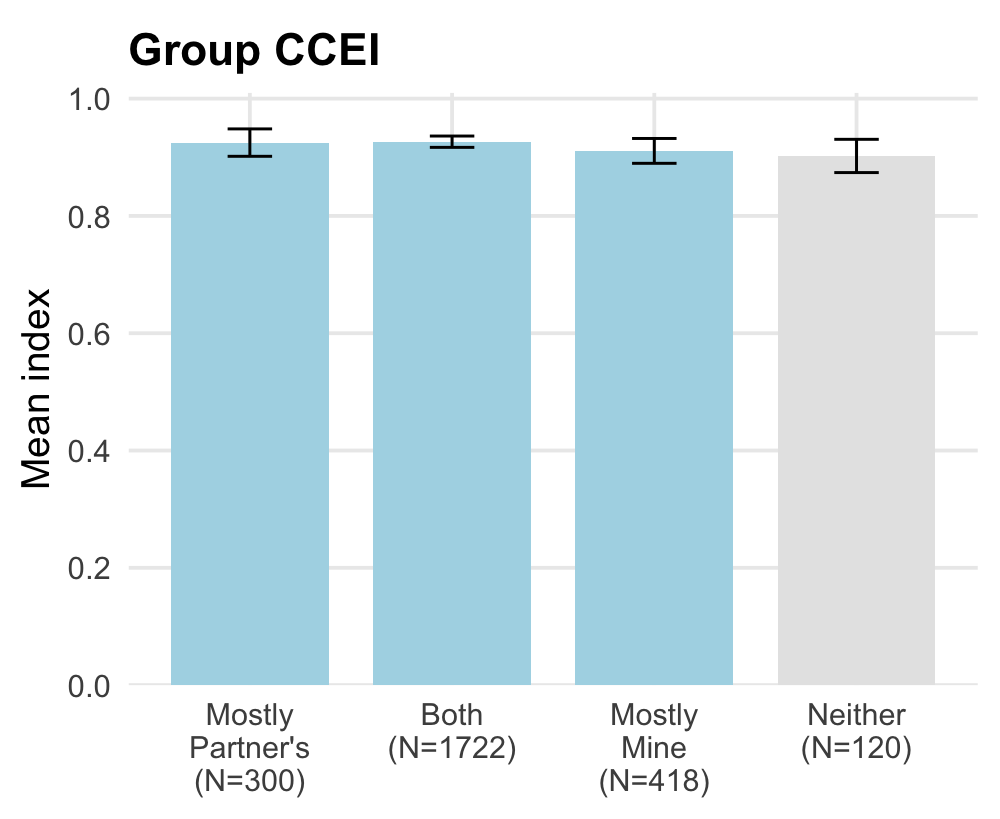
\includegraphics[width=0.326\textwidth]{whose.common.ccei_g.png}
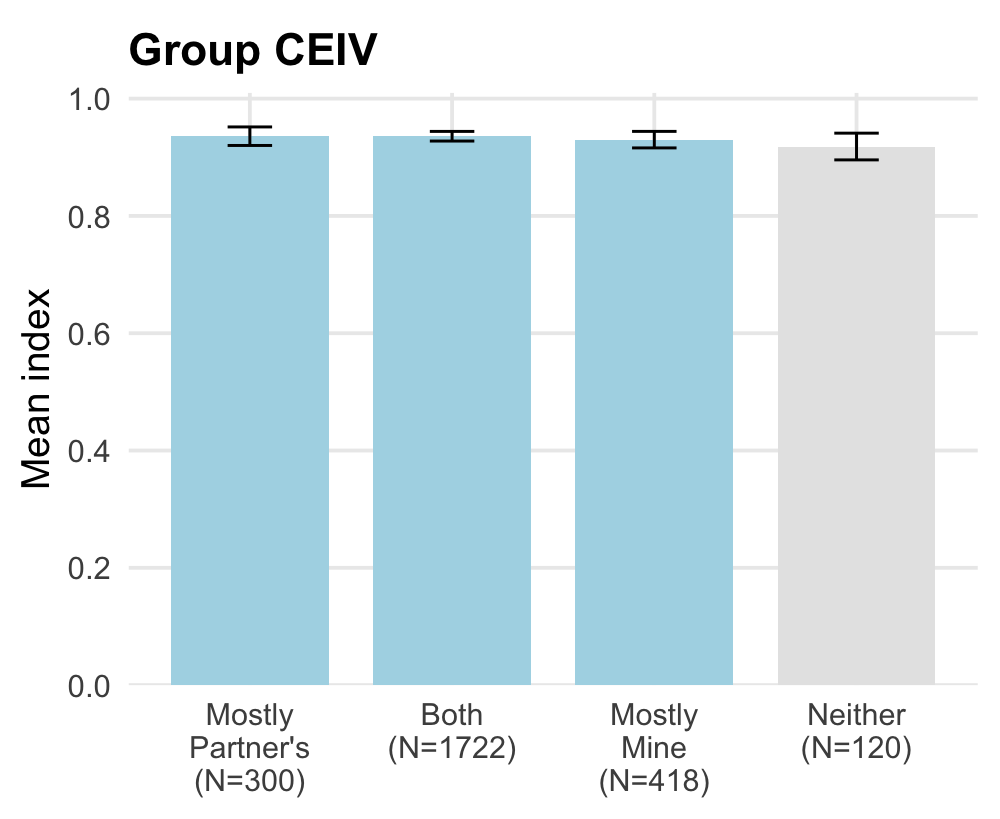
\includegraphics[width=0.326\textwidth]{whose.common.ceiv_g.png}
\end{center}
\small
Survey: During the collective choice experiment, whose suggestions were most reflected in the final choices? The Neither category is shaded gray, following Figure 5.

\textit{Notes:} Means and 95\% confidence intervals clustered by 64 classes. All three panels use the same 2,560 respondent-wave observations (1,280 pair-waves). Group CCEI and CEIV are shared by the two members; plots sort them by each member's own survey response. Counts therefore refer to respondents, not independent groups. All panels use a common 0--1 scale.

\textbf{Reading the pattern.} The preference-distance bars and counts reproduce Figure 5(a). Group outcomes vary much less clearly across these reports; the full-sample categorical tests give p=0.098 for CCEI and p=0.339 for CEIV.

Preference distance is the current raw normalized $I_{ig}$ used in Figure 5, with lower values indicating greater alignment. Within each pair-wave, the two defined distances sum to one; it is a relative member-to-group measure, not an absolute measure of group quality. The 48 observations without distance are excluded from these plots, while the summary correlations use all available observations for each outcome.
\clearpage
\begin{center}\Large\textbf{Similarity among pairs with high risk-preference disagreement}\par
\normalsize Figure 5(b) sample restriction\end{center}
\begin{center}
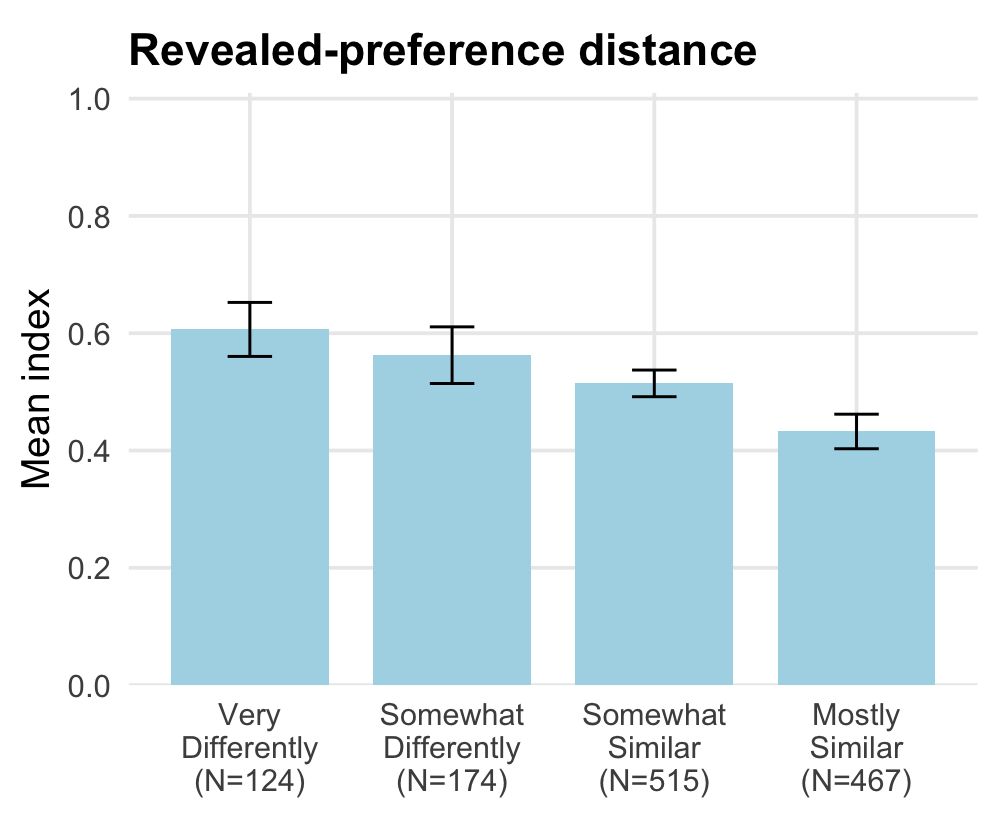
\includegraphics[width=0.326\textwidth]{similar.high_gap.distance.png}
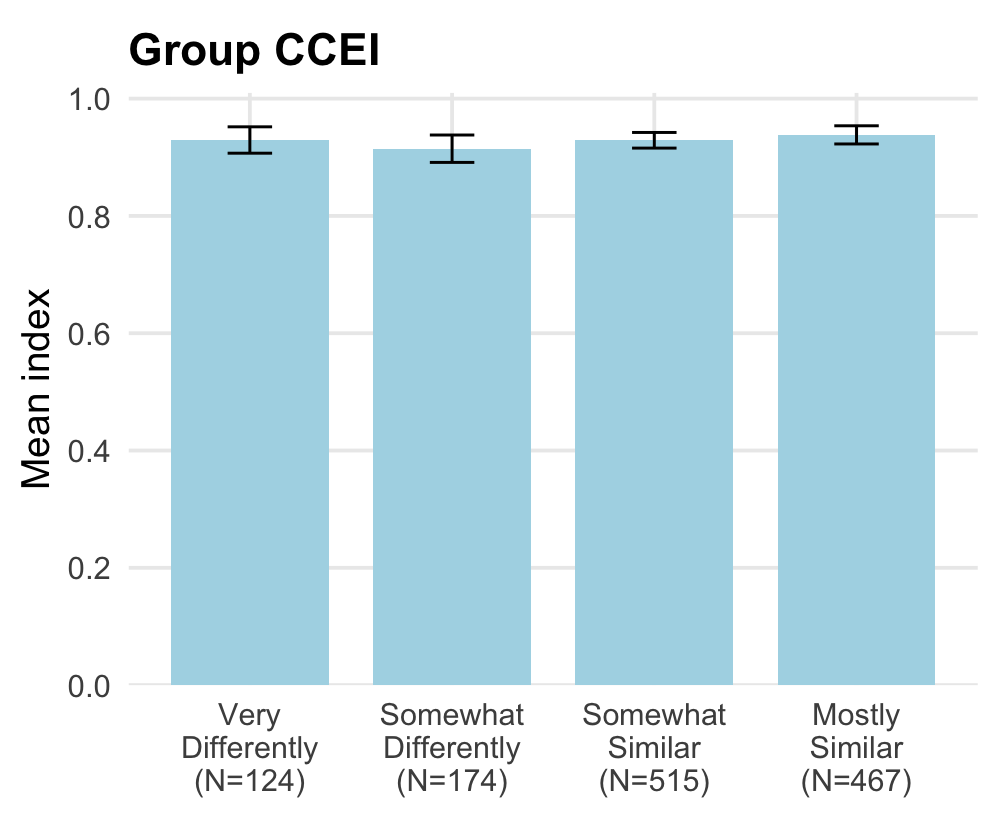
\includegraphics[width=0.326\textwidth]{similar.high_gap.ccei_g.png}
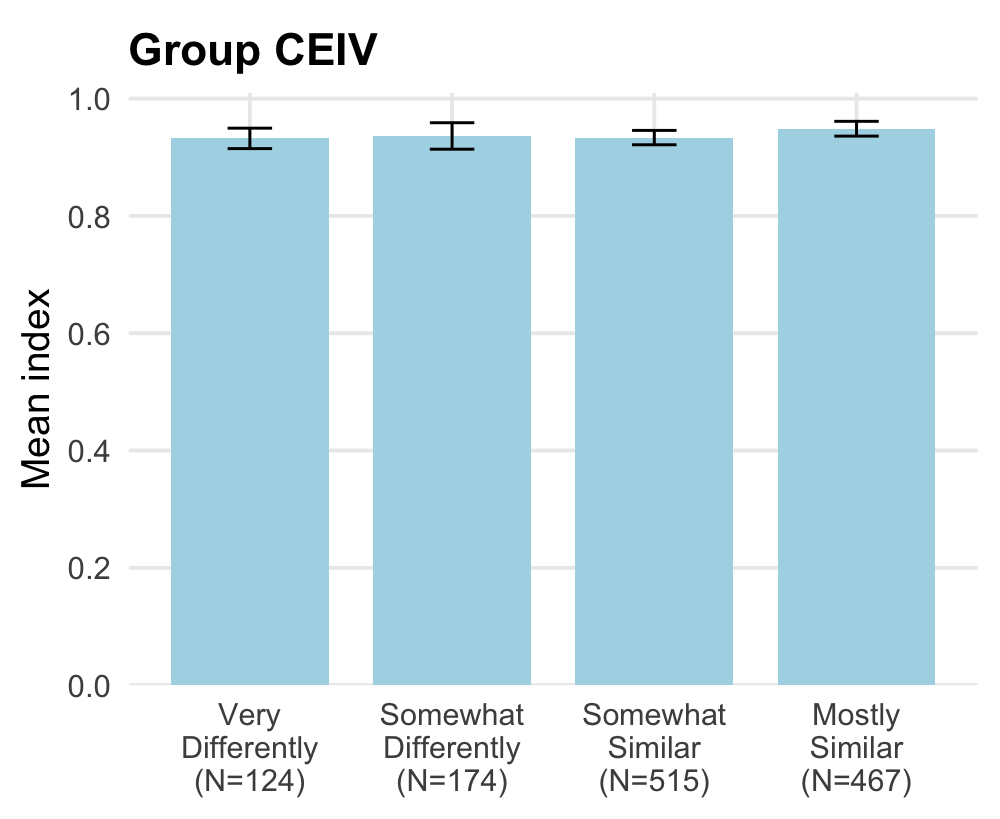
\includegraphics[width=0.326\textwidth]{similar.high_gap.ceiv_g.png}
\end{center}
\small
This reproduces Figure 5(b)'s restriction: the pair's absolute individually revealed risk-preference gap is at or above the pooled median in the distance-observed sample (0.126720506). It is not the wave-specific median split used in the separate heterogeneity exercise.

\textit{Notes:} Means and 95\% confidence intervals clustered by 64 classes. All three panels use the same 1,280 respondent-wave observations (640 pair-waves). Group CCEI and CEIV are shared by the two members; plots sort them by each member's own survey response. Counts therefore refer to respondents, not independent groups. All panels use a common 0--1 scale.

\textbf{Reading the pattern.} The distance relationship is stronger in this subgroup. Mean group outcomes show weaker linear gradients than in the full sample; rank correlations remain positive. See the checks below.

\begin{center}\begin{tabular}{lrrr}\toprule Outcome & Pearson $r$ ($p$) & Spearman $\rho$ ($p$) & Adjusted slope ($p$)\\\midrule
Preference distance & -0.169 ($<0.001$) & -0.172 ($<0.001$) & -0.064 ($<0.001$)\\
Group CCEI & 0.043 (0.123) & 0.108 ($<0.001$) & 0.006 (0.115)\\
Group CEIV & 0.049 (0.068) & 0.072 (0.010) & 0.005 (0.117)\\
\bottomrule\end{tabular}\end{center}
\end{document}
